\section{In painting}
  We have discussed the importance of good input data, and the potential benefits to resource usage and ease of making a good model.
  So a priority when it comes to image classification is to have data without anomalies and other areas that can be interpreted as a feature for the classifier. 
  In a machine learning perspective, the data is best if it has the same structure, and is %TODO similar enough.
  In painting is the process of reconstructing lost or deteriorated parts of images and videos. %TODO CITE https://en.wikipedia.org/wiki/Inpainting
  

  From prior papers on polyp detection in the GI tract %TODO CITE!!!
  we have clear results that the black corners, and the green squares trigger a big activation %TODO WRITE BETTER
  when it comes to classifying images. 
  From %TODO CITE, find out who
  's paper, we can see that the activation map on a regular image gives very high result on, in addition to the polyp, the corners and the green sqare. 
  \begin{figure}[h]
    \centering
    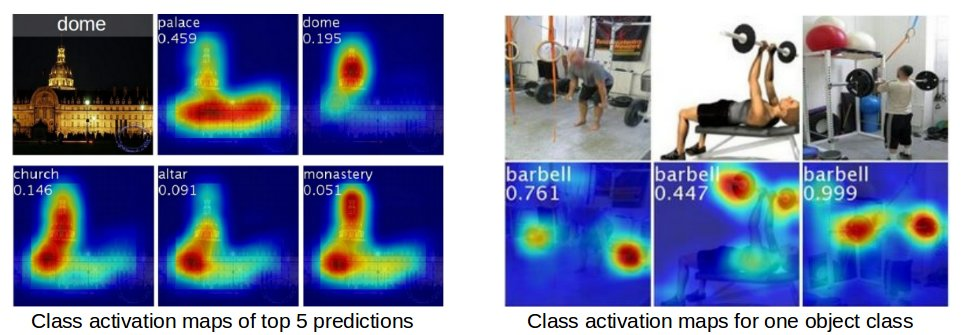
\includegraphics[scale=0.5]{background/figures/placeholder.jpeg}
    \caption{Using X's activation map we can see that the edges triggers unwanted activations}
  \end{figure}
  
  In addition to sqares and edges, we also have the problem that parts of the image is over saturated at points where the light from the led is reflected directly back to the camera.
  Another problem is when the camera captures images that are too close to the wall. Both of these scenarios creates patches where the saturation is maximum. 
   \begin{figure}[h]
    \centering
    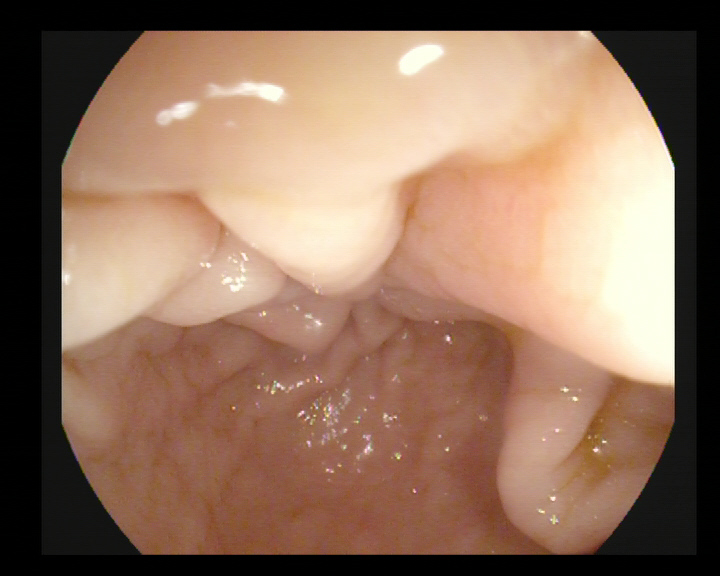
\includegraphics[scale=0.5]{background/figures/reflection.jpg}
    \caption{we have two different types of saturation: the reflected area in the top part of the image, and the right side of the image.}
  \end{figure}
  in an ideal scenario the image would have no pixel values at max, and as little frame as possible. 
  We therefor want to make a tool that can help us with this.
  \subsection{Naive methods for In painting}
    Inpainting is not a new area of research, as it has been around since %TODO CITE
    Because of this there are many naive methods that gives good inpaintings. 
	
    \subsubsection{Textured syntesys based on image inpainting}
    \subsubsection{MOARE}
    \subsubsection{MOARE}
	
    As we can see from this, there are a lot of old methods that can give approximations. We can also conclude that none of these methods are perfect.
    We will therefore look at methods that takes learning in to use.
  \subsection{Using machine learning for inpainting}
    As discussed earlier, machine learning is using prior experiences to make dessisions given the problem at hand. 
    It is also worth mentioning that we do not need labeled data, since we are in a way looking at a global average of every image both with, and without polyps. We are therefor insetiviced to use an 
    Unsupervised approach.
    Since machine learning is learning from a training set, it is important that the training set contains as little as possible of the features we want to remove. \\
    
    Because of this the first thing we need to do if we are going to mask out corners and sqares, is to limit the training set to only contain cropped, non-sqare images. 
 
    \begin{figure}[ht]
      \centering
      \begin{minipage}[b]{0.45\textwidth}
	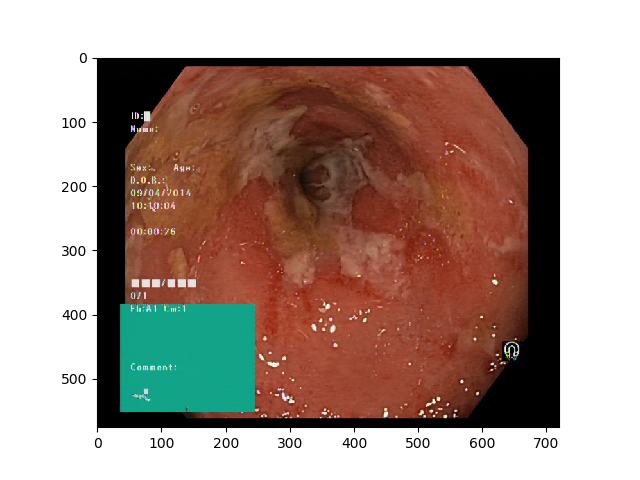
\includegraphics[width=\textwidth]{background/figures/uncropped_img.png}
	\caption{Original image with black padding}
      \end{minipage}
      \hfill
      \begin{minipage}[b]{0.45\textwidth}
	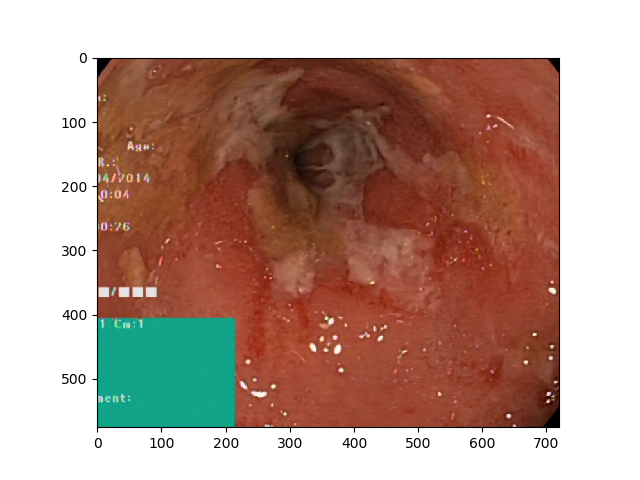
\includegraphics[width=\textwidth]{background/figures/cropped_8percent_img.png}
	\caption{Black edges cropped away + 8\% zoom}
      \end{minipage}
      \caption{Here we have an example on how we would make an image better to train on. This is not representative of the training, since we only use images without the green square under training}
    \end{figure}
    
    Now that we have better images to train our data with, we need the correct algorithm.
    We have already seen unsupervised learning aproaches in chapter %TODO ref 
    \subsubsection{Algorithm}
      \todo{Hvordan skal jeg gaa frem nar det kommer til aa presantere disse? skal jeg bare si hvilke metoder jeg har testet?}
      Text about presenting UML, and stuff.
      \subsubsection{Autoencoder}
      
      \subsubsection{Contextencoder}
      \subsubsection{CCgan}
      \subsubsection{PixelCNN}
      
  
 
